\chapter{Artifact Design} \label{chap_designing_artifacts}

This chapter will discuss specific design decisions made to meet the required
functionality while adhering to the requirements outlined in chapter
\ref{chap_requirements}. Two different artifacts are used to support this study. Figure
\ref{fig_overview_design} is a schematical overview of both these artifacts.

The first artifact consists of two main components: the Clean Architecture Expander and
the Expander framework. The name of the Expander Framework, Pantha Rhei, was inspired by
the Greek philosopher \emph{Heraclitus}, who famously stated that \enquote{life is flux.}
The name reflects the artifact's perceived ability to cope with constant change in a
stable and evolvable manner. Users can interact with the Expander Framework using the
\gls{cli} command \enquote*{flux} in combination with several parameters. Appendix
\ref{appendix_run_flux}, yprovides a comprehensive guide on using this command, including
all available options and parameters.



\begin{figure}[H]
    \centering
    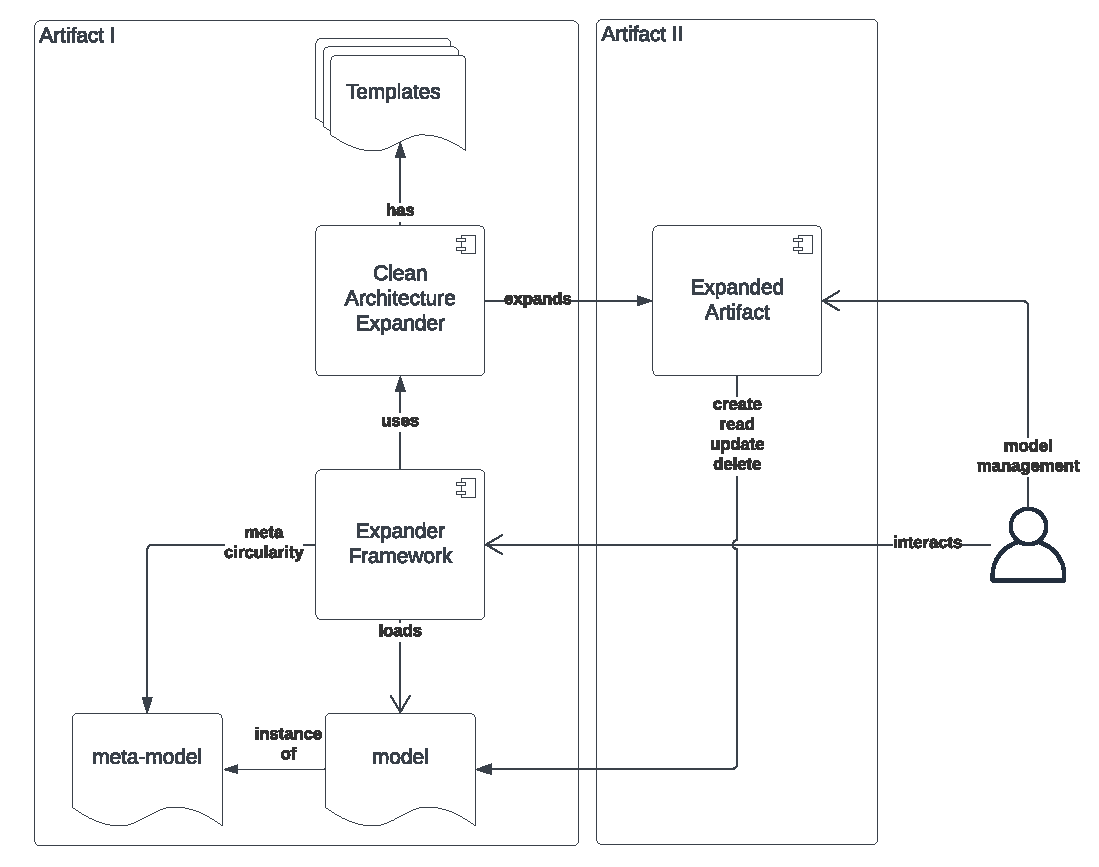
\includegraphics[width=0.8\textwidth]{figures/artifactOverview.pdf}
    \caption[Schematic overview of the Artifacts]{Schematic overview of the Artifacts}
    \label{fig_overview_design}
  \end{figure}

  As illustrated in Figure \ref{fig_overview_design}, the main task of the first artifact
  or \enquote*{expand} the second artifact. By entering the correct command, the Expander
  Framework loads the model being instantiated during the expansion process. Then, the
  required expanders are prepared based on information available through the model. In the
  case of this study, the Clean Architecture Expander. The Clean Architecture Expander
  consists of a set of tasks and templates. When the Expander Framework executes the Clean
  Architecture Expander, the model is instantiated into the generated artifact with the
  aid of the templates.

  The model is an instance of the meta-model. Consequently, the model can represent any
  application as long as the meta-model is respected. In the case of this study, the model
  represents the entities, attributes, relationships, and other characteristics of the
  meta-model.
  
  As a result, the second artifact (artifact II) allows a user to modify or maintain the
  model used by the Expander Framework by exposing a Restful interface. This method
  approaches the meta-circularity process, where an expansion process is used to
  update the meta-model. Although not fully compliant with the theory of \gls{ns}, the
  Expander Framework consists of the required tasks to update its own meta-model. This is
  illustrated in Figure \ref{fig_overview_design} by the \enquote*{updates} arrow.

\section{The Artifact name and use} \label{sec_artifact_name}

The name of the Expander Framework, Pantha Rhei, was inspired by the Greek philosopher
\emph{Heraclitus}, who famously stated that \enquote{life is flux}. The name reflects the
artifact's ability to cope with constant change in a stable and evolvable manner. The name
is also reflected in the use of the \enquote{flux} command in the \gls{cli}, which allows
users to interact with the application.

To install Pantha Rhei, interested readers can follow the instructions provided in the
appendix \fullref{koks_installation_2023}.





\chapter{The Entity Relationship Diagram of the Meta Mode} \label{appendix_metamodel_description}  

\section{The App entity}

The App entity represents the application and is regarded as the entry point for the
model. The App Entity and the subsequent entities contain all the information required to
perform the expandsion of a software system. 

\begin{table}[H]
    \small
    \begin{tabular}{ p{0.21\linewidth} p{0.21\linewidth} p{0.49\linewidth} }
        \hline
        \textbf{Name} & \textbf{DataType} & \textbf{Description} \\
        \hline
        Id & Guid & Unique identifier of the application \\
        Name & string & Name of the application \\
        FullName & string & Full name of the application \\
        Expanders & List of Expanders & The Expanders that will be used during the
        generation process. \\
        Entities & List of Entities & The Entities that are applicable for the Generated artifact. \\
        ConnectionStrings & List of ConnectionStrings & The ConnectionString to the
        database that is used by the Generator Artifact. \\
        \hline
    \end{tabular}
    \caption{The fields of the App entity}
    \label{table:app_entity}
\end{table}

\section{The Component entity}

The Component entity represents a software component that can be part of an application.
Based on this entity the Generator Artifact can make design time on where to place certain
elements  

\begin{table}[H]
\small
\begin{tabular}{ p{0.20\linewidth} p{0.20\linewidth} p{0.50\linewidth} }
\hline
\textbf{Name} & \textbf{DataType} & \textbf{Description} \\
\hline
Id & Guid & Unique identifier of the component \\
Name & string & Name of the component \\
Description & string & Description of the component \\
Packages & List of Package & The Packages that should be applied to the component. \\
Expander & Expander & Navigation property to the Expander entity. \\
\hline
\end{tabular}
\caption{The fields of the Component entity}
\label{table:component_entity}
\end{table}

\section{The ConnectionString entity}

The ConnectionString entity represents a ConnectionString used by an application to
connect to a database or other external system.

\begin{table}[H]
\small
\begin{tabular}{ p{0.20\linewidth} p{0.20\linewidth} p{0.50\linewidth} }
\hline
\textbf{Name} & \textbf{DataType} & \textbf{Description} \\
\hline
Id & Guid & Unique identifier of the ConnectionString \\
Name & string & Name of the ConnectionString \\
Definition & string & Definition of the ConnectionString \\
App & App & Navigation property to the App entity \\
\hline
\end{tabular}
\caption{The fields of the ConnectionString entity}
\label{table:connectionstring_entity}
\end{table}

\section{The Entity entity}

The Entity entity represents an entity in the application's data model. 

\begin{table}[H]
\small
\begin{tabular}{ p{0.20\linewidth} p{0.23\linewidth} p{0.47\linewidth} }
\hline
\textbf{Name} & \textbf{DataType} & \textbf{Description} \\
\hline
Id & Guid & Unique identifier of the entity \\
Name & string & Name of the entity \\
Callsite & string & The source code location where the entity is defined. In the case of a C\#
artifact, this is to determine the name of the namespace.\\
Type & string & Type of the entity \\
Modifier & string & Modifier of the entity (e.g. public, private) \\
Behavior & string & The behavior of the entity (e.g. abstract, virtual) \\
App & App & Navigation property to the App entity. \\
Fields & List of Fields & The Fields property represents a collection of the fields that
make up the entity. \\
ReferencedIn & List of Fields & Represents a navigation property to a Field that uses the
current entity as a return type. \\
Relations & List of Relationships & List of relationships involving this entity \\
IsForeignEntityOf & List of Relationships & List of relationships where this entity is the foreign entity \\
\hline
\end{tabular}
\caption{The fields of the Entity entity}
\label{table:entity_entity}
\end{table}

\section{The Expander entity}

The Expander entity represents an expander, which is responsible for generating code for
an application. The Generator Artifact attempts to execute all expanders that are related
to the selected App.

\begin{table}[H]
\small
\begin{tabular}{ p{0.20\linewidth} p{0.22\linewidth} p{0.48\linewidth} }
\hline
\textbf{Name} & \textbf{DataType} & \textbf{Description} \\
\hline
Id & Guid & Unique identifier of the expander \\
Name & string & Name of the expander \\
TemplateFolder & string & relative path to the templates that are used by the expander. \\
Order & int & The order in which the expander is executed \\
Apps & List of Apps & List of applications associated with the expander. \\
Components & List of Components & List of components associated with the expander \\
\hline
\end{tabular}
\caption{The fields of the Expander entity}
\label{table:expander_entity}
\end{table}

\section{The Field entity}

The Field entity represents a field or property of an entity in an application's data
model. Each field has a unique ID, name, and other properties such as its return type,
modifiers, and behavior. It can be associated with an entity and can have relationships
with other entities. The IsKey and IsIndex properties indicate whether the field is part
of the primary key or an index of the entity, respectively.

\begin{table}[H]
\small
\begin{tabular}{ p{0.23\linewidth} p{0.23\linewidth} p{0.45\linewidth} }
\hline
\textbf{Name} & \textbf{DataType} & \textbf{Description} \\
\hline
Id & Guid & Unique identifier of the field \\
Name & string & Name of the field \\
ReturnType & string & Return type of the field \\
IsCollection & bool & Whether the field is a collection or not \\
Modifier & string & Modifier of the field (e.g. public, private) \\
GetModifier & string & Modifier of the get accessor for the field \\
SetModifier & string & Modifier of the set accessor for the field \\
Behavior & string & The behavior of the field (e.g. abstract, virtual) \\
Order & int & The order of the field within its entity \\
Size & int? & The size of the field \\
Required & bool & Whether the field is required or not \\
Reference & Entity & The entity that this field refers to\\
Entity & Entity & A navigation property to the parent entity \\
IsKey & bool & Indicates whether the field is part of the primary key \\
IsIndex & bool & Indicates whether the field is part of an index \\
RelationshipKeys & List of Relationships & A List of entities that are defined as relations. \\
IsForeignEntityKeyOf & List of Relationships & List of relationships to the field that is the foreign key \\
\hline
\end{tabular}
\caption{The fields of the Field entity}
\label{table:field_entity}
\end{table}

\section{The Package entity}

The Package entity represents a software package that can be used by a component. This
could either be a Nuget package in the case of .NET projects, or for example npm packages
for web projects.

\begin{table}[H]
\small
\begin{tabular}{ p{0.20\linewidth} p{0.20\linewidth} p{0.50\linewidth} }
\hline
\textbf{Name} & \textbf{DataType} & \textbf{Description} \\
\hline
Id & Guid & Unique identifier of the package \\
Name & string & Name of the package \\
Version & string & Version of the package used \\
Component & Component & Component associated with the package \\
\hline
\end{tabular}
\caption{The fields of the Package entity}
\label{table:package_entity}
\end{table}

\section{The Relationship entity}

The Relationship entity represents a relationship between two entities in the App's data
model. The Relationship entity has proper cardinality support. Relationships are
bidirectional and can be navigated from either entity.

\begin{table}[H]
\small
\begin{tabular}{ p{0.24\linewidth} p{0.12\linewidth} p{0.55\linewidth} }
\hline
\textbf{Name} & \textbf{DataType} & \textbf{Description} \\
\hline
Id & Guid & Unique identifier of the relationship \\
Key & Field & The key field of the relationship \\
Entity & Entity & Navigation property to the parent Entity \\
Cardinality & string & The cardinality of the relationship \\
WithForeignEntityKey & Field & The foreign key field of the relationship, pointing to a
Field entity. \\
WithForeignEntity & Entity & The entity associated with the foreign key field \\
WithCardinality & string & The cardinality of the relationship with the foreign entity \\
Required & bool & indicates whether the relationship is required or not \\
\hline
\end{tabular}
\caption{The fields of the Relationship entity}
\label{table:relationship_entity}
\end{table}
\section{Plugin Architecture} \label{subsec_plugin_architecture}

The Expander Framework Artifact is responsible for loading and bootstrapping Expanders and
initiating the generation process. Expanders are dynamically loaded at runtime through a
dotnet capability called assembly binding, allowing the architecture illustrated in the
following image \parencite{koks_expanderpluginloaderinteractor_2023}.

\begin{figure}[H]
  \centering
  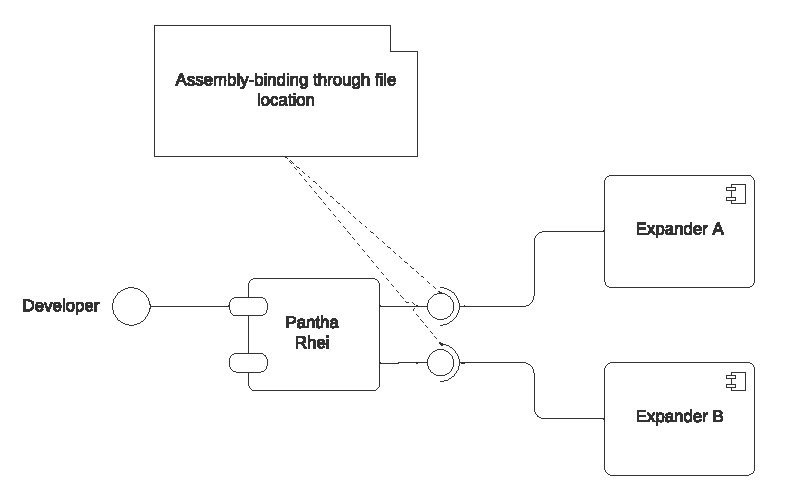
\includegraphics[width=0.5\textwidth]{figures/plugin_architecture.pdf}
  \caption[Plugin Archticture]{Expanders are considered plugins}
  \label{fi:plugin_architecture}
\end{figure}

This plugin design adheres to several principles of \gls{solid}. The \gls{srp} principle
is implemented by ensuring that an expander generates one and only one construct. The
\gls{ocp} principle is applied by allowing the creation of new expanders in addition to
the already existing ones. The \gls{lsp} principle is respected by enabling the addition
or replacement of expanders without modifying the internal workings of the Expander
Framework.

More details can be found in the Appendix \fullref{list_expanderpluginloaderinteractor}
\section{Expanders}

The Exander Framework allows for the miscellaneous execution of expanders of any type. The
Expander Framework is independent of any of the details of Expanders, fully adhering to
the principle of \gls{dip}. Conversely, an Expander is required to implement several
interfaces to ensure execution and dependency management are available during runtime. The
Expander Framework also consists of a set of default tasks, such as the execution of the
expansion tasks known as ExpanderHandlerInteractors
\citecode{koks_iexpanderhandlerinteractor_2023}, logging, bootstrapping dependencies, and
tasks to execute harvestings and injections. Except for the use of the
IExpanderInteractor, non of which are required.

Figure \ref{fig_expander_design} illustrates the dependencies between the domain layer of
the Expander Framework. The Clean Architecture Expander is considered an application layer
containing specific tasks bounded to a particular application or process. In this case,
the Expansion process.

\begin{figure}[H]
    \centering
    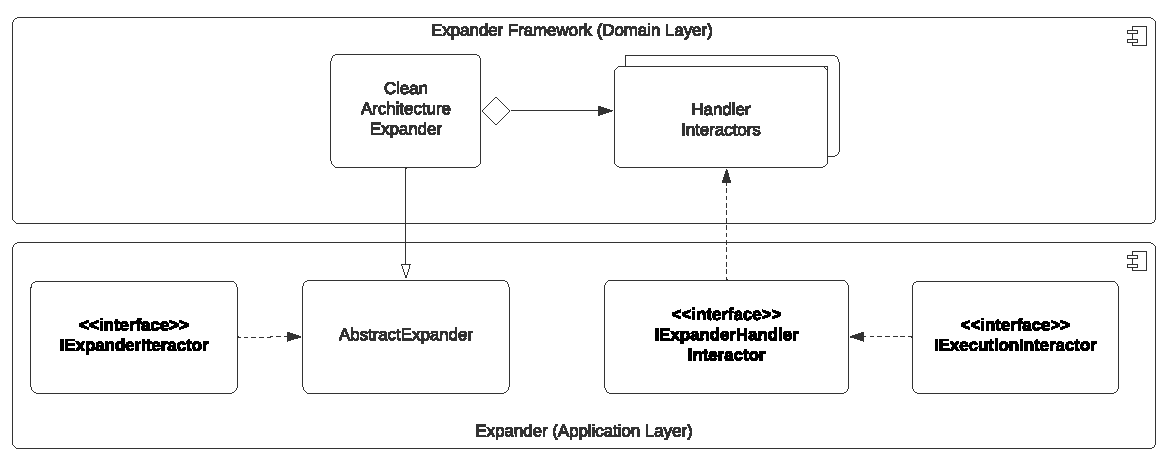
\includegraphics[width=1\textwidth]{figures/expander.pdf}
    \caption[The design of an Expander]{The design of an Expander}
    \label{fig_expander_design}
  \end{figure}
\section{The IExecutionInteractor command} \label{subsec_IExecutionInteractorObject}

An exciting implementation that facilitates a high degree of cohesion while maintaining
low coupling is the utilization of the \code{koks_iexecutioninteractor_2023} interface
\parencite{koks_iexecutioninteractor_2023}. This interface allows for the execution of
various derived types responsible for specific tasks, such as executing Handlers,
Harvesters, and Rejuvenators \parencites{koks_expandentitieshandlerinteractor_2023,
koks_regionharvesterinteractor_2023, koks_regionrejuvenatorinteractor_2023}. The
implementation promotes decoupling by adhering to both \gls{ocp} and \gls{lsp}.

\begin{figure}[H]
    \centering
    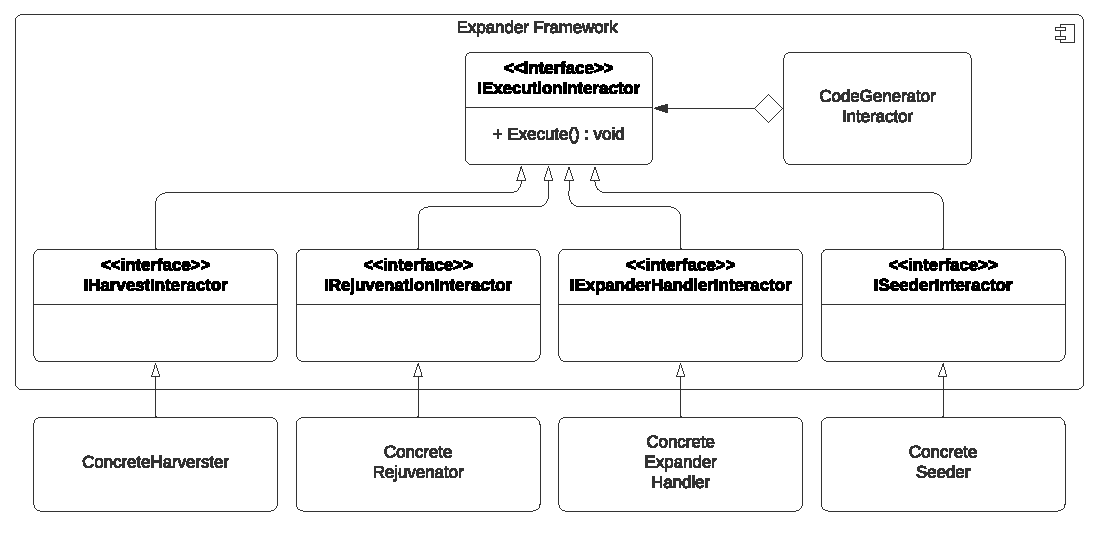
\includegraphics[width=1\textwidth]{figures/command_pattern.pdf}
    \caption[Low coupling with \code{koks_iexecutioninteractor_2023}]{Low coupling with \code{koks_iexecutioninteractor_2023}}
    \label{fig_iexecutioninteractor}
  \end{figure}


Figure \ref{fig_iexecutioninteractor} illustrates that the required interfaces are placed
in the Domain Layer of the Expander Framework. In contrast, the concrete classes also can
be implemented as part of the internal scope of the Clean Architecture Expander
\parencite{koks_migrationharvesterinteractor_2023}. Code listing
\fullref{list_expandentitieshandlerinteractor} illustrates an implementation example of
this interface. Finally, the code listing \fullref{list_CodeGeneratorInteractor}
illustrates the aggregation of the execution, which allows for a graceful cohesion of the
execution Tasks \parencite{koks_codegeneratorinteractor_2023}.

\section{Dependency management}

\begin{enumerate}
    \color{red}
    \item TODO: DESCRIBE DI and use of service locator pattern.
\end{enumerate}